\documentclass[12pt]{article}

\usepackage[utf8]{inputenc}
\usepackage[T1]{fontenc}
\usepackage{graphicx}
\usepackage[french]{babel}
\usepackage[top=3cm, bottom = 3cm, right = 3cm, left = 3cm]{geometry}
\usepackage{amssymb}
\usepackage{amsmath}
\usepackage{stmaryrd}
\usepackage{hyperref}
\usepackage[ruled,vlined]{algorithm2e}

\usepackage{tikz}
\usetikzlibrary{positioning,chains,fit,shapes,calc}

\definecolor{myred}{RGB}{160,80,80}
\definecolor{mygreen}{RGB}{80,160,80}
\definecolor{myblue}{RGB}{80,80,160}
\definecolor{problem}{RGB}{80,80,250}

\begin{document}

%\maketitle
\begin{titlepage}
    ~ \vfill
    \begin{center}
      \LARGE  Université de Bordeaux - Master 2\\[1.5cm]

      {\Large \bfseries \bsc{--- Algorithmique appliquée ---}}\\[0.5cm]

      \rule{\linewidth}{0.5mm}\\[0.4cm] {\Huge \bfseries Projet stratégies de défense à la RoboCup \\[0.2cm]} \rule{\linewidth}{0.5mm}\\[1.5cm] {
      \Large Adrien \bsc{Maurin}, Florian \bsc{Simba}}\\[0.5cm]

                {\large Encadré par Ludovic \bsc{Hofer}}\\ \vfill
                
\includegraphics[width = 300px]{logo.jpg} \vfill
                                {\large 18 novembre 2020}
    \end{center}
\end{titlepage}

\section{Définition formelle du problème}

\subsection{Input}

\paragraph{Les constantes}

\begin{itemize}
  \item $p_{step}$ : il s'agit de la valeur qui indique l'écart minimal entre deux positions possibles pour des défenseurs. Cela permet de discrétiser $\mathbb{R}^2$. On a alors $p_{step} \in \mathbb{R}^*_+$.
  \item $\theta_{step}$ : il s'agit de la valeur minimale de l'angle qui doivent former deux droites pour ne pas être confondues. Cela permet de discrétiser les angles (compris dans $]-\pi ; \pi]$).
  \item $r$ : il s'agit du rayon des cercles qui modélisent les robots. On a alors $r \in \mathbb{R}^*_+$.
\end{itemize}

\paragraph{Limites du terrain} Le terrain de jeu est un rectangle délimité par deux points $(x_{min}, y_{min})$ et $(x_{max}, y_{max})$. Il s'agit donc de l'ensemble de points $F$ tels que :

\begin{equation*}
F = [x_{min}, x_{max}] \times [y_{min}, y_{max}].
\end{equation*}

\paragraph{Le terrain} Le terrain est modélisé par l'ensemble de points $T$ tel que :

\begin{equation*}
T = \{ (x, y) \in F \ |\  x \equiv 0 \bmod p_{step} \wedge y \equiv p_{step} \bmod 0 \}.
\end{equation*}

Autrement dit, il s'agit de la grille de points contenant l'origine du plan et dont la taille des cases est de $p_{step}$.

\paragraph{Les robots} Les robots sont modélisés par l'ensemble de points suivants avec $p_0$ le point central du robot :

\begin{equation*}
    R_{p_0} = \{ p \in \mathbb{R}^2 \ |\  ||p_0 - p|| \leqslant r \}.
\end{equation*}


\paragraph{Les positions des attaquants} Il s'agit d'un ensemble de points représentant les points centraux des attaquants tel que :
\label{section:size_team}
\begin{equation*}
    A = \{ p \in F \}.
\end{equation*}

Le cardinal de l'ensemble $A$ est par ailleurs borné par le nombre d'attaquants. Selon les règles officielles de la RoboCup Small Size League (SSL)\footnote{\url{https://ssl.robocup.org/}}, les équipes ne peuvent pas excéder 8 joueurs. On a ainsi $|A| \leqslant 8$. On suppose dans ce problème qu'il existe au moins un attaquant pour que le problème soit intéressant.

Une propriété que doit satisfaire les attaquants est qu'il ne doit pas y avoir de collisions lors de leur placement :

\begin{equation*}
\forall i, j \in \llbracket 1, |A| \rrbracket, i \ne j, \neg collision(a_i, a_j)
\end{equation*}

La fonction $collision$ peut être exprimée de la manière suivante :

\begin{align*}
  collision \colon &F^2 \to \{0, 1 \}\\
  &d_i, d_j \mapsto collision(d_i, d_j) = \begin{cases}
                                   0 & \text{si $|| d_i - d_j || < 2r$ } \\
                                   1 & \text{sinon.}
  \end{cases}
\end{align*}

\paragraph{Le(s) goal(s)} Il s'agit d'un ensemble de segments délimités par deux points. Un dernier paramètre permet d'indiquer le sens du goal, i.e. par quel \og côté \fg{} du segment la droite de tir doit passer. On notera ce vecteur $g$. Le segment délimitant le goal sera noté $G$.

\paragraph{Les tirs des attaquants} Il s'agit d'un ensemble $B$ de demi-droites représentant les tirs tel que :

\begin{equation*}
    B = \{ (p_0, \theta) \in F \times ]-\pi: \pi] \ | \ p_0 \in A \wedge \theta \equiv 0 \bmod \theta_{step} \}.
\end{equation*}

\paragraph{Les tirs cadrés}
Pour qu'un tir soit cadré, il faut que le tir d'un attaquant traverse le segment du goal dans le bon sens (le produit scalaire entre le vecteur du goal et celui de la droite de tir est strictement négatif). Cette représentation montre les tirs qui atteignent le but sans prendre en compte les défenseurs. L'ensemble $B_c$ des tirs cadrés est exprimé ainsi :

\begin{equation*}
    B_c = \{ b \in B \ | \ , b \cap G \ne \emptyset \wedge (b|g) < 0  \}
\end{equation*}


\paragraph{Les tirs non-cadrés}
Pour qu'un tir soit non-cadré, il faut que le tir d'un attaquant ne traverse pas le segment du goal, ou dans le mauvais sens sinon. Il s'agit du complémentaire de l'ensemble précédent. L'ensemble $B_{nc}$ est exprimé ainsi :

\begin{equation*}
    B_{nc} = B \textbackslash B_c
\end{equation*}

\subsection{Output}

\paragraph{Les positions des défenseurs} Il s'agit d'un ensemble de points $p_i$ dans $D$ tels que :

\begin{equation*}
D = \{ \forall i, j \in \llbracket 1, |D| \rrbracket, i \ne j, \neg collision(d_i, d_j) \wedge B = \emptyset \}.
\end{equation*}

Le cardinal de l'ensemble $D$ est par ailleurs borné par le nombre de défenseurs comme défini en section \ref{section:size_team}. On a ainsi $|D| \leqslant 8$.

\section{Modélisation du problème}

On va modéliser le problème que l'on vient de définir de manière formelle comme un problème de graphe.

\subsection{Construction du graphe}

\paragraph{Les n\oe uds représentant les tirs}
Un tir est est une combinaison entre la position d'un attaquant et un angle $(p_0, \theta)$. On ne considère que les tirs cadrés. Pour chaque tir cadré, on lui associe un n\oe ud sur notre graphe. On note l'ensemble de ces sommets $V_t$.

\paragraph{Les n\oe uds représentant les position des défenseurs}
La position d'un défenseur est modélisée par un point du terrain. On ne considère que les positions disponibles, i.e. l'ensemble des points de $G$ qui ne sont pas en collision avec au moins un élément de $A$. Pour chaque position de défenseur, on lui associe un n\oe ud sur notre graphe. On note l'ensemble de ces sommets $V_d$.

\paragraph{} L'ensemble des sommets du graphe est alors égal à $V = V_t \cup V_d$.

\paragraph{Les interceptions}
Une interception entre un tir et un défenseur est modélisée comme une arête reliant le tir d'un attaquant à une position de défenseur. On note cet ensemble $E$. Le graphe que l'on obtient est alors biparti entre l'ensemble de n\oe uds $V_d$ et $V_t$.

\subsection{Simplification du graphe}
On simplifie le graphe que l'on vient d'obtenir en retirant les sommets isolés (correspondant à des positions de défenseurs n'interceptant aucun tir).

\subsection{Résolution du problème}
Résoudre le problème initial, i.e. trouver le nombre minimal de défenseurs permettant de défendre le but se ramène dans notre modélisation à résoudre le problème de graphe suivant :

\paragraph{Problème} \textcolor{problem}{Il faut trouver le plus petit sous ensemble de $V_d$ tel que cet ensemble domine $V_t$.}

\subsection{Exemple d'application}

La figure \ref{tikz:example} montre un exemple de la modélisation du problème. Ici, il existe 5 trajectoires de tirs permettant aux adversaires de marquer. On dispose de 5 emplacements pour placer nos défenseurs.  On constate que placer un défenseur à la position $Def_1$ et un défenseur à la position $Def_4$ permet de bloquer la totalité des tirs (les arêtes en bleu). L'ensemble des tirs est alors dominé par notre groupe de défenseurs. On remarque dans cet exemple qu'on ne peut pas faire mieux que 2 défenseurs.


\begin{figure}[h!]
\centering
\label{tikz:example}
\begin{tikzpicture}[thick,
  every node/.style={draw,circle},
  fsnode/.style={fill=myred},
  ssnode/.style={fill=mygreen},
  every fit/.style={ellipse,draw,inner sep=-2pt,text width=2cm},
  -,shorten >= 3pt,shorten <= 3pt
]

% the vertices of U
\begin{scope}[start chain=going below,node distance=7mm]
\foreach \i in {1,2,...,5}
  \node[fsnode,on chain] (f\i) [label=left: $Tir_\i$] {};
\end{scope}

% the vertices of V
\begin{scope}[xshift=6cm,start chain=going below,node distance=7mm]
\foreach \i in {1,2,...,5}
  \node[ssnode,on chain] (s\i) [label=right: $Def_\i$] {};
\end{scope}

% the set U
\node [myred,minimum size = 4cm, fit=(f1) (f5),label=above:Tirs cadrés] {};
% the set V
\node [mygreen, minimum size = 4cm, fit=(s1) (s5),label={[align=center]above:Positions des\\ défenseurs}] {};

% the edges
\draw[myblue, line width = 0.5mm] (f1) -- (s1);
\draw[myblue, line width = 0.5mm] (s1) -- (f2);
\draw (f2) -- (s2);
\draw (s3) -- (f3);
\draw[myblue, line width = 0.5mm] (f3) -- (s4);
\draw[myblue, line width = 0.5mm] (s4) -- (f4);
\draw[myblue, line width = 0.5mm] (f5) -- (s1);
\draw (s5) -- (f4);
\draw (f2) -- (s3);
\end{tikzpicture}
\caption{Exemple du problème où les 5 tirs sont bloqués par deux défenseurs 1 et 4.}
\end{figure}

\subsection{Interception de tir}
Un tir étant défini à l'aide d'un angle $\theta$ et d'un point $(x_0, y_0)$. Pour déterminer si ce dernier est intercepté par un point, on peut dans un premier retrouver l'équation de la demi-droite :

\begin{align*}
y & =  y_0 + (x - x_0)\tan \theta & \text{ et $x \geqslant x_0$ si } \theta \in ]-\frac{\pi}{2}; \frac{\pi}{2} [ \\
y & = y_0 + (x - x_0)\tan \theta & \text{ et $x \leqslant x_0$ si } \theta \in ]-\pi; \frac{\pi}{2}[ \cup ]\frac{\pi}{2}; \pi ] \\
x & = x_0  & \text{ et $y \geqslant 0$ si } \theta = \frac{\pi}{2} \\
x & = x_0  & \text{ et $y \leqslant 0$ si } \theta = -\frac{\pi}{2} \\
\end{align*}

Une fois que l'on a l'équation de la demi-droite modélisant le tir, pour vérifier s'il y a une interception d'un tir à une position d'un défenseur on calcule la distance minimale entre la demi-droite de tir et le point position du défenseur. Cette distance est calculée à partir de la formule suivante :

\begin{equation*}
  d = \frac{|Ax_0 + By_0 + C|}{\sqrt{A^2+B^2}}
\end{equation*}

avec $Ax+By+C = 0$ l'équation de la droite et $(x_0, y_0)$ la position du défenseur.

 Si cette distance est inférieure à $R$ (rayon du robot), alors le tir est intercepté.

\subsection{Récupération des positions}

Les figures \ref{figure:terrain_placements} et \ref{figure:terrain_tirs} permettent de voir les positions du terrain qui sont utilisées dans notre graphe par rapport aux tirs des attaquants. Dans cet exemple, l'algorithme a compté 75 tirs cadrés parmis les 300 tirs possibles. Ensuite, l'algorithme a gardé dans le graphe 726 positions qui interceptaient des tirs parmis les 5 400 positions disponibles.

\begin{figure}[h!]
  \centering
  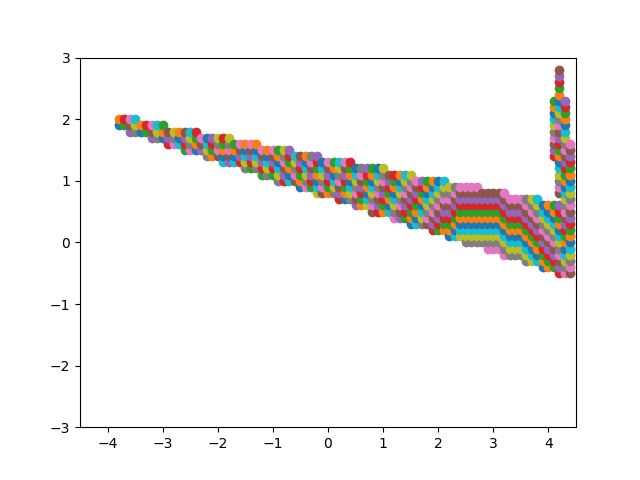
\includegraphics[width = 13cm]{terrain_placements.png}
  \caption{Exemple de carte des positions interceptant les tirs.}
  \label{figure:terrain_placements}
\end{figure}

\begin{figure}[h!]
  \centering
  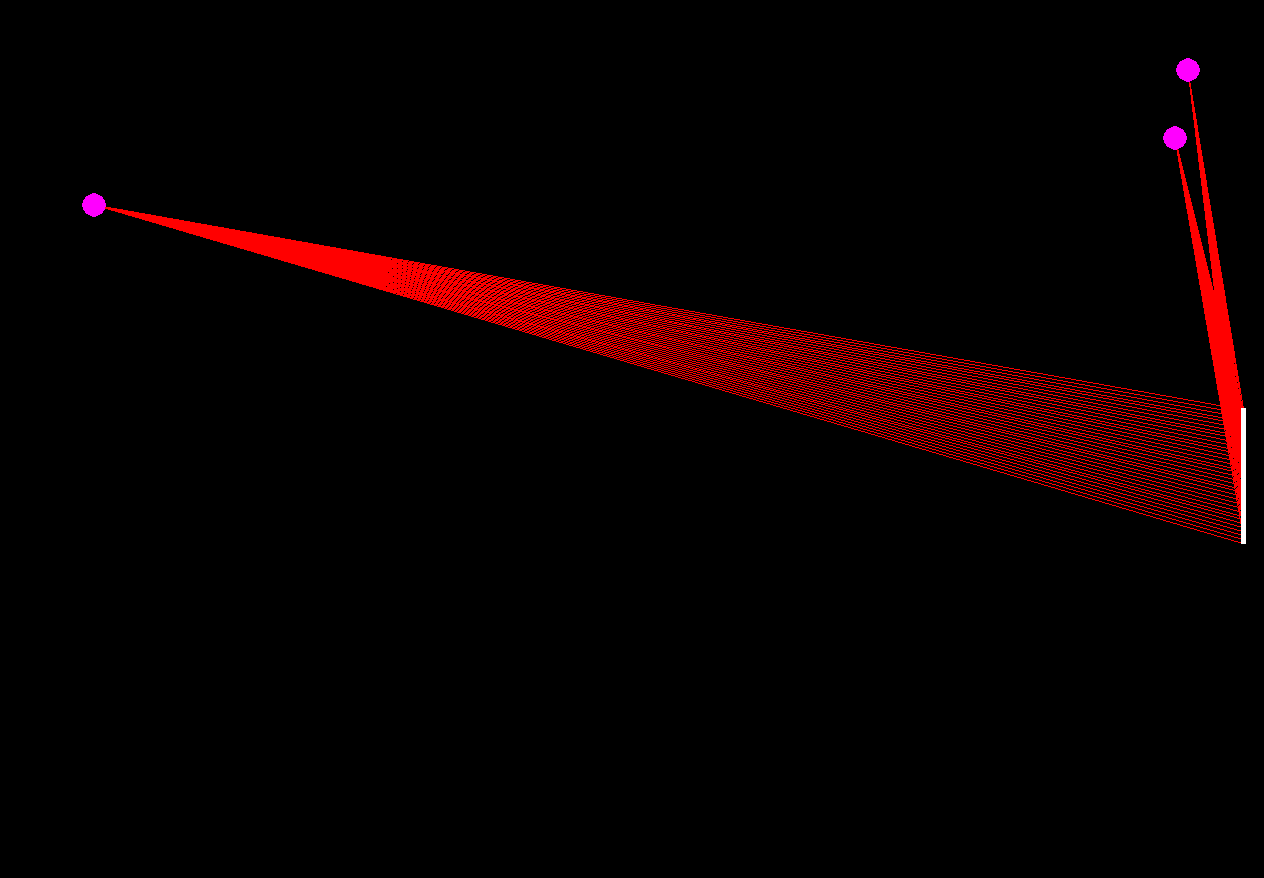
\includegraphics[width = 13cm]{terrain_tirs.png}
  \caption{Exemple de carte des tirs sur le même problème.}
  \label{figure:terrain_tirs}
\end{figure}

\newpage

\section{Pistes de résolution du problème}

Cette section présente différents algorithmes de résolution à notre problème ; l'algorithme exhaustif et l'algorithme glouton.


\subsection{Utilisation d'un algorithme exhaustif}

\paragraph{Fonctionnement général}
Pour résoudre le problème d'ensemble dominant dans notre graphe, on peut dans un premier temps utiliser un algorithme exhaustif, qui, pour toute configuration d'ensemble de sommets dans $V_d$, vérifie si elle est dominante ou non. L'avantage est qu'on aura la meilleure solution possible.

\paragraph{Notre algorithme}
On commence par énumérer les configurations avec $k=1$ défenseur. Si on trouve une configuration qui résout notre problème, on retourne l'ensemble dominant les tirs. Sinon, on énumère  les configurations avec $k=2$ défenseurs. On continue jusqu'à atteindre $k=8$. Si on ne trouve pas de solution pour $k = 8$, la configuration ne peut pas être défendue.

\begin{figure}[h!]
  \begin{algorithm}[H]
    \SetKw{Continue}{continue}
    \SetKw{Function}{Function}
    \SetKwBlock{Deb}{begin}{end}
    \Function{exhaustif(G, k, D = $\emptyset$)}
    \BlankLine
    \KwResult{D un ensemble dominant}
    \Deb{
    \If{k = 0}{
      \If{isDominated(Vt(G), D)}{
        \Return D \;
      } {
        \Return $\emptyset$ \;
      }
    }
    \For{i in Vd(G)}{
      \If{i in D}{
        \Continue \;
      } {
        E = exhaustif(G, k - 1, D $\cup$ i) \;
        \If{E != $\emptyset$} {
          \Return E \;
        }
      }
    }
    \Return $\emptyset$ \;}
  \end{algorithm}
  \caption{Implémentation de notree algorithme exhaustif.}
\end{figure}

\newpage

\paragraph{Complexité} Vérifier si le sous-ensemble $D$ est un ensemble dominant peut se faire en temps $\mathcal{O}(n+m) = \mathcal{O}(n^2)$\footnote{En réalité, on ne regardera seulement les sommets de $V_t$ et les arêtes entre notre solution $D$ et $V_t$. Cette borne est assez large et il est possible de l'affiner.}, avec $n = |V(G)|$ et $m = |E(G)|$. Pour savoir si un ensemble $D$ de taille $k$ domine les tirs, il faut un temps de :

\begin{equation*}
  \binom{n}{k} \dot\  \mathcal{O}(n^{2}) = \mathcal{O}(n^{k+2})
\end{equation*}

Comme $k$ peut aller jusqu'à 8, on a une complexité en $\mathcal{O}(n^{10})$. Cependant, la complexité de cet algorithme dépend beaucoup de l'ensemble dominant que l'on trouve ($\mathcal{O}(n^{2+|D|})$). Il peut ainsi être intéressant de tester des configurations avec beaucoup de défenseurs pour défendre.

Le désavantage de cet algorithme est le coût en temps qui, si le nombre minimal de défenseur nécessaire est grand ($k \geqslant 4$), peut être problématique pour obtenir une solution rapidement. Par ailleurs, un trop grand nombre de sommets modélisant des tirs ou des positions d'interception peuvent aussi rendre plus difficile la résolution du problème.

\subsection{Utilisation d'un algorithme glouton}

\paragraph{Fonctionnement général} Pour résoudre le problème d'ensemble dominant dans notre graphe, on utilise ensuite l'algorithme glouton. On cherche un ensemble de sommets de taille $k$ qui domine l'ensemble des tirs. On va choisir pour cela un sommet dominant le plus de sommets de tir non dominés. On continue jusqu'à ce qu'on ait trouvé un ensemble dominant ou atteint la taille maximum de l'ensemble.

Avec cet algorithme, il est possible que la solution qu'on obtienne ne soit pas optimale.


\paragraph{Notre algorithme}

\begin{figure}[h!]
  \begin{algorithm}[H]
    \SetKw{Continue}{continue}
    \SetKw{Function}{Function}
    \SetKwBlock{Deb}{begin}{end}
    \Function{glouton(G, k, D = $\emptyset$)}
    \BlankLine
    \KwResult{D un ensemble dominant}
    \Deb{
    \If{isDominated(Vt(G), D)}{
      \Return D \;
    }
    \If{k = 0}{
        \Return $\emptyset$ \;
      }
    i = mostDominatePos(G, D) \;
    E = glouton(G, k - 1, D $\cup$ i) \;
    \Return E \;
    }
  \end{algorithm}
  \caption{Implémentation de notre algorithme glouton.}
\end{figure}

La fonction \texttt{mostDominatePos} renvoie le sommet qui domine le plus de sommets de tirs non dominés par des sommets de l'ensemble $D$.

\paragraph{Complexité} Pour chaque sommet de position, on va compter son degré en soustrayant les sommets déjà dominés. La complexité est en $\mathcal{O}(|V_t||D|)$ puisque pour chaque élément de $D$, on vérifie quels sont les sommets de tirs qu'il domine. On en arrive à une complexité de $\mathcal{O}(|V_t||D||V_d|)$. On fait cet appel de fonction au plus $|D|$ fois. On obtient une complexité de $\mathcal{O}(|V_t||D|^2|V_d|)$. Le cas terminal comme pour l'algorithme exhaustif se fait en $\mathcal{O}(n+m)$. Comme la taille de $D$ est au plus de 8, et $V_t$ et $V_d$ sont majorés par le nombre de sommets total $n$, on obtient une complexité en $\mathcal{O}(n^2)$.

\section{Extensions : fonctionnalités développées et envisagées}

Cette section présente les avantages et inconvénients de notre modélisation par rapport aux extensions à développer.

\paragraph{Plusieurs buts}
On a réussi à implémenter cette fonctionnalité dans l'algorithme exhaustif. S'il y a plusieurs buts, le nombre de trajectoires ne fera que s'accroître. Si $V_{ti}$ correspond aux tirs cadrés dans le goal $i$ et qu'il y a $n$ buts, alors $V_t = V_{t1} \cap \cdots \cap V_{tn}$.


\paragraph{Position initiale des joueurs} Nous n'avons pas encore implémenté cette fonctionnalité, mais nous donnons des informations pour la résolution d'un tel problème dans la suite.

Dans le cas ou la position initiale des défenseurs est connue, on peut introduire un paramètre $movestep$ qui symbolise la distance maximale qu'un défenseur peut parcourir pour intercepter le tir. Les changements dans notre modèle sont les suivants :

\begin{itemize}
  \item Les positions des défenseurs ne sont plus tous les points de $G \textbackslash A$ mais tous les points du terrains à portée de déplacement des défenseurs.
  \item Pour chaque ensemble de sommet à portée de chaque défenseur, on transforme cette ensemble en clique (on ajoute toutes les arêtes possibles entre les sommets de l'ensemble).
\end{itemize}

La solution doit ensuite dominer l'ensemble des tirs mais aussi l'ensemble des defenseurs.

\paragraph{Distance minimale entre les robots} Nous n'avons pas encore implémenté cette fonctionnalité, mais nous donnons des informations pour la résolution d'un tel problème dans la suite.

Dans le cas ou les robots nécessitent de respecter une distance minimale, nous pouvons introduire un paramètre $D$ modélisant la distance minimale de deux robots.

Pour prendre en compte cette contrainte, il faut légèrement changer notre modélisation. À partir du sous-graphe $G'$ comportant les sommets $V_d$, on place une arête entre deux sommets si les positions des défenseurs sont à une distance inférieure à $D$. La solution de positionnement des défenseurs doit être un stable de $G'$.


\paragraph{Gardien}
On a réussi à implémenter cette fonctionnalité dans l'algorithme exhaustif.

Pour pouvoir prendre en compte cette extension dans notre modèle, il faut prendre en compte les modifications suivantes :
\begin{itemize}
  \item L'ensemble des sommets de position des défenseurs situés dans le goal est égal à $V_g$. L'ensemble des sommets $V$ du graphe est alors égal à $V_t \cup V_g \cup V_d$.
  \item On place des arêtes entre des sommets de $V_t$ et $V_d$ et entre des sommets de $V_t$ et $V_g$ s'il y a des interceptions de tir.
\end{itemize}

La solution de positionnement des défenseurs ne doit autoriser le placement que d'un unique défenseur dans le goal (un seul sommet dans $V_g$).
Lors de l'énumération des configurations, on a un booléen qui indique si un sommet de $V_g$ a déjà été utilisé dans l'ensemble que l'on regarde. Si oui, alors on choisit aléatoirement un sommet parmis les sommets de $V_d$ sinon, on choisit aléatoirement un sommet parmis les sommets de $V_d \cup V_g$.

Par ailleurs, cette méthode peut aussi produire des solutions ou il y a 0 défenseur dans le terrain du goal.

\paragraph{Trajectoires courbées}
Cette extension n'est pas encore prise en compte par nos algorithmes mais peut être envisagée.

Pour pouvoir gérer des trajectoires courbées, on peut maintenant dire que les tirs sont modélisés par des polynômes et non des droites. L'équation de la trajectoire devient alors $y = ax^2 bx + c$ contrairement à $y = bx+c$. Par ailleurs, désactiver cette extension revient à fixer $a$ à 0. Le paramètre $a_{max}$ sera ajusté en fonction de l'importance de la courbure des tirs. Par exemple, pour des tirs avec une faible courbure on prendra $a_{max}$ petit et pour des tirs avec une courbure importante on prendra $a_{max}$ grand.

Lors du calcul des trajectoires des tirs cadrés, il ne faudra pas seulement prendre en compte les tirs rectilignes mais aussi les tirs courbées avec un niveau de courbure variable. Supposons que l'on ait un paramètre $a_{step}$, alors on calcule toutes les équations de courbe avec $a \in [0, a_{max}] \wedge a \equiv 0 \bmod a_{step}$.

Cette extension ne nécessite pas vraiment de changements dans notre modélisation à part à lors des calculs d'interception de tirs. Cela aura tendance à augmenter le nombre de sommets modélisant des tirs, mais la résolution de l'algorithme reste similaire.

\section{Critique des performances}

Nous avons effectué les mesures suivantes sur une machine possédant les caractéristiques suivantes :

\begin{itemize}
  \item Processeur : Intel(R) Core(TM) i7-9750H CPU @ 2.60GHz
  \item Ram : 16 GB
  \item OS : Linux machine virtuelle
\end{itemize}

En utilisant la commande \texttt{time} du terminal, nous avons récupéré le temps de l'exécution de l'algorithme. Ce temps comprends notamment la lecture des données d'entrée (fichier JSon) ainsi que la construction d'une structure de graphe et la résolution du problème.

Par soucis d'implémentation, nous n'avons pas encore pu réaliser les mesures de temps de l'algorithme glouton.

\begin{center}
  \begin{tabular}{|l|c|c|}
    \hline
    & Algorithme exhaustif & Algorithme glouton \\
    \hline
    Problème de base 1 & 0.165 & / \\
    \hline
    Problème de base 2 & 0.126 & / \\
    \hline
    Extension multigoal & 0.207 & / \\
    \hline
    Extension gardien & 0.126 & / \\
    \hline
  \end{tabular}
\end{center}

On obtient des résultats de l'ordre du dixième de seconde pour l'algorithme exhaustif. Ces résultats semblent réalistes au sens où durant la partie, pouvoir récupérer les informations des robots (position, cages, etc.) et organiser la défense doit prendre peu de temps par rapport à la vitesse du ballon.

%\section{Proposition de modification de la formalisation du problème}



\end{document}
